%%%%%%%%%%%%%%%%%%%%%%%%%%%%%%%%%%%%%%%%%%%%%%%%%%%%%%%%%%%%%%%%%%%%%%%%%%%%%%%
%
% witseiepaper-2005.tex
%
%                       Ken Nixon (12 October 2005)
%
%                       Sample Paper for ELEN417/455 2005
%
%%%%%%%%%%%%%%%%%%%%%%%%%%%%%%%%%%%%%%%%%%%%%%%%%%%%%%%%%%%%%%%%%%%%%%%%%%%%%%%%

\documentclass[10pt,twocolumn]{witseiepaper}
%
% All KJN's macros and goodies (some shameless borrowing from SPL)
\usepackage{KJN}
\usepackage[super]{nth}
\usepackage{subcaption}
\usepackage{listings}
\usepackage{amsmath,amsfonts,amssymb}
\usepackage{epstopdf}
\usepackage{xcolor}
\usepackage{textcomp}
\usepackage{listings}
\usepackage{alltt}
%\usepackage{matlab-prettifier}
\usepackage{graphicx}
\usepackage{changes}
\usepackage{makecell}
\usepackage{verbatim}
\usepackage{balance}
\usepackage{pdfpages}
\usepackage{ragged2e}
\usepackage{algorithm}
\usepackage{algorithmicx}
\usepackage{multirow}
\usepackage[noend]{algpseudocode}
\usepackage{color} %red, green, blue, yellow, cyan, magenta, black, white
\definecolor{mygreen}{RGB}{28,172,0} % color values Red, Green, Blue
\definecolor{mylilas}{RGB}{170,55,241}
%\usepackage{flafter}

%
% PDF Info
%
\ifpdf
\pdfinfo{
	/Title (INSTRUCTIONS AND STYLE GUIDELINES FOR THE PREPARATION OF FINAL YEAR LABORATORY PROJECT PAPERS : 2005 VERSION)
	/Author (Ken J Nixon)
	/CreationDate (D:200309251200)
	/ModDate (D:200510121530)
	/Subject (ELEN417/455 Paper Format, 2005)
	/Keywords (ELEN417, ELEN455, paper, instructions, style guidelines, laboratory project)
}
\fi

%%%%%%%%%%%%%%%%%%%%%%%%%%%%%%%%%%%%%%%%%%%%%%%%%%%%%%%%%%%%%%%%%%%%%%%%%%%%%%%
\begin{document}
	
	\begin{titlepage}
		
		\newcommand{\HRule}{\rule{\linewidth}{0.3mm}} % Defines a new command for the horizontal lines, change thickness here
		
		\center % Center everything on the page
		
		%----------------------------------------------------------------------------------------
		%	HEADING SECTIONS
		%----------------------------------------------------------------------------------------
		
\includegraphics[width=0.3\textwidth]{EIE.png}\\[1cm] % Include a department/university logo - this will require the graphicx package
		
		%----------------------------------------------------------------------------------------
		\textsc{\LARGE University of the Witwatersrand } \\[0.1cm] % Name of your university/college
		\textsc{\LARGE School of Electrical and Information Engineering }\\[1cm] % Major heading such as course name
		\textsc{\Large ELEN4020: Data Intensive Computing}\\[1.5cm] % Minor heading such as course title
		
		%----------------------------------------------------------------------------------------
		%	TITLE SECTION
		%----------------------------------------------------------------------------------------
		
		\HRule \\[0.4cm]
		{ \huge \bfseries Laboratory Exercise 2} \\[0.4cm] % Title of your document
		\HRule \\[1.5cm]
		
		%----------------------------------------------------------------------------------------
		%	AUTHOR SECTION
		%----------------------------------------------------------------------------------------
		\textsc{\Large 	\emph{Authors:} } \\[0.1cm]	 
		
		
		\begin{minipage}{0.4\textwidth}
			\begin{flushleft} \large
				%			\emph{Author:} \\
				Kayla-Jade Butkow \\ 714227 % Your name
			\end{flushleft}
		\end{minipage}
		~
		\begin{minipage}{0.4\textwidth}
			\begin{flushright} \large
				%	\emph{Author:}\\
				Jared Ping \\ 704447
			\end{flushright}
		\end{minipage}\\[1cm]
		
		\begin{minipage}{0.4\textwidth}
			\begin{flushleft} \large
				%		\emph{Author:}\\
				Lara Timm \\ 704157
			\end{flushleft}
		\end{minipage}
		~
		\begin{minipage}{0.4\textwidth}
			\begin{flushright} \large
				%		\emph{Author:} \\
				Matthew van Rooyen \\ 706692
			\end{flushright}
		\end{minipage}\\[1cm]
		
		
		
		{\large Date Handed In: \nth{9} March, 2018}\\[1cm] 
		
	\end{titlepage}


\pagestyle{plain}
\setcounter{page}{1}
\onecolumn
%%%%%%%%%%%%%%%%%%%%%%%%%%%%%%%%%%%%%%%%%%%%%%%%%%%%%%%%%%%%%%%%%%%%%%%%%%%%%%%
%
\section{Matrix Transposition}
In order to allow for simple matrix transposition, the two-dimensional square matrix is created as a one-dimensional array, populated in row-major form. The one-dimensional array is filled with integer values, where the value is equal to the $index + 1$.

To ensure efficiency, only the lower left triangle of the matrix is traversed. This is sufficient as in matrix transposition the middle diagonal remains unchanged while each entry in the lower triangle is swapped with a single entry in the upper triangle. For each position in the lower triangle, the index of the entry with which that integer should be swapped is calculated using Equation~\ref{newIndexEqn}~\cite{inPlaceTranspose}.

\begin{equation}
\label{newIndexEqn}
index_{old} = (index_{new}*N)~mod(N^2-1)
\end{equation}

To ensure that the matrix is transposed in place, a traditional style swap function, making use of integer pointers, is implemented.

\section{OpenMP}
The multi-threaded algorithm was implemented using OpenMP. Multi-threading was performed on all aspects of the process, including the populating of the matrix and the transposition of the array. 

For all of the processes using OpenMP, the loops were divided into chunks of the size of the matrix divided by 256. Each function takes in a parameter called \texttt{noOfThreads}, which allows the user to specify the number of threads that should be used to execute the process.

Since the matrix is large, populating it in serial takes a large amount of time. It was thus implemented in parallel. Since each loop takes a consistent amount of time (as the same process is performed in each loop), static scheduling was used \cite{HPC}. 

The transposition was also performed using static scheduling, as it proved to give the best performance. 

\section{PThreads}
The multi-threaded algorithm was implemented using POSIX Threads (PThreads). Multi-threading was performed on all aspects of the process, including the populating of the matrix and the transposition of the array. 

The PThreads library offers a much lower level approach in implementing parallelism, offering high performance at the cost of substantial source code modification and code maintainability. This is noted when comparing the source code length of the OpenMP implementation to that of the PThreads implementation.

In comparison to the OpenMP implementation, it can be seen that required work per thread is specified when each thread is created as opposed to continuously feeding chunks of data to each thread \cite{pthread}. This translates to a significant performance increase as the dataset scales. Each function takes in a parameter called \texttt{noOfThreads}, which allows the user to specify the number of threads that should be used to execute the process.

The general process of PThread implementation involves correctly dividing up the required work based on the number of specified threads, thereafter initialising each thread and assigning it the appropriate work. An important component is to always ensure the threads synchronise after completing the specified workload.

Thread functions were implemented, which are non-returning pointer functions that are provided as arguments for a thread's workload. These functions only accept a single argument and thus structs were created to pass all relevant data which the thread required to complete the assigned workload.

\section{Comparison of Performance}

\begin{table}[h]
	\centering
	\caption{Performance of the algorithm when run as a serial process (measured in seconds)}
	\begin{tabular}{|c|c|c|}
	\hline
	  N$_{0}$ = N$_{1}$ = 128 &  N$_{0}$ = N$_{1}$ = 1024 & N$_{0}$ = N$_{1}$ = 8192 \\
		\hline 
		0.000270  & 0.010812 & 1.609882 \\ 
		\hline 
	\end{tabular} 
\end{table} 

\begin{table}[h]
\centering
\caption{Performance of the algorithm using 4 threads (measured in seconds)}
\begin{tabular}{|c|c|c|c|}
	\hline 
	 & N$_{0}$ = N$_{1}$ = 128 &  N$_{0}$ = N$_{1}$ = 1024 & N$_{0}$ = N$_{1}$ = 8192 \\ 
	\hline 
	PThread & 0.000175 & 0.004886 & 0.766117 \\ 
	\hline 
	OpenMP & 0.000138 & 0.011894 & 1.649183 \\ 
	\hline 
\end{tabular}
\end{table} 

\begin{table}[h]
		\centering
\caption{Performance of the algorithm using 8 threads (measured in seconds)}
\begin{tabular}{|c|c|c|c|}
	\hline 
	 & N$_{0}$ = N$_{1}$ = 128 &  N$_{0}$ = N$_{1}$ = 1024 & N$_{0}$ = N$_{1}$ = 8192 \\ 
	\hline 
	PThread & 0.000184 & 0.003155 & 0.532490 \\ 
	\hline 
	OpenMP & 0.000207 & 0.010809 & 1.665707 \\ 
	\hline 
\end{tabular} 
\end{table}

\begin{table}[h]
		\centering
	\caption{Performance of the algorithm using 16 threads (measured in seconds)}
\begin{tabular}{|c|c|c|c|}
	\hline 
	 & N$_{0}$ = N$_{1}$ = 128 &  N$_{0}$ = N$_{1}$ = 1024 & N$_{0}$ = N$_{1}$ = 8192 \\ 
	\hline 
	PThread & 0.000418 & 0.002654 & 0.476413 \\ 
	\hline 
	OpenMP & 0.000168 & 0.012843 & 1.623063 \\ 
	\hline 
\end{tabular} 
\end{table}

\begin{table}[h]
		\centering
	\caption{Performance of the algorithm using 64 threads (measured in seconds)}
\begin{tabular}{|c|c|c|c|}
	\hline 
	 & N$_{0}$ = N$_{1}$ = 128 &  N$_{0}$ = N$_{1}$ = 1024 & N$_{0}$ = N$_{1}$ = 8192 \\ 
	\hline 
	PThread & 0.001417 & 0.002739 & 0.482428 \\ 
	\hline 
	OpenMP & 0.000573 & 0.012632 & 1.655354 \\ 
	\hline 
\end{tabular} 
\end{table}

\begin{table}[h]
	\centering
	\caption{Performance of the algorithm using 128 threads (measured in seconds)}
	\begin{tabular}{|c|c|c|c|}
		\hline 
		& N$_{0}$ = N$_{1}$ = 128 &  N$_{0}$ = N$_{1}$ = 1024 & N$_{0}$ = N$_{1}$ = 8192 \\ 
		\hline 
		PThread & 0.002326 & 0.003241 & 0.448408 \\ 
		\hline 
		OpenMP & 0.001360 & 0.011724 & 1.620541 \\ 
		\hline 
	\end{tabular} 
\end{table}

\begin{figure} [htbp]
	\centering
	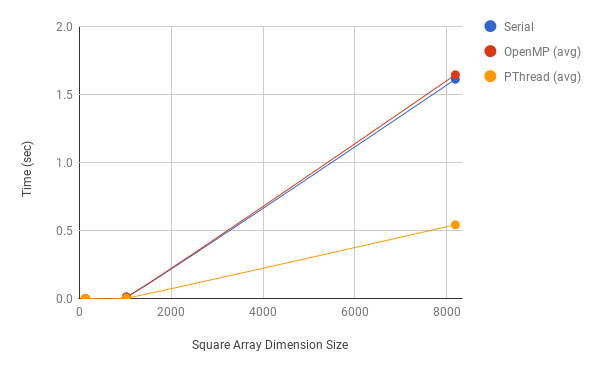
\includegraphics[width=\textwidth]{benchmark}
	\caption{Performance benchmark of transposition algorithm.}
	\label{fig:benchmark}
\end{figure}

%%%%%%%%%%%%%%%%%%%%%%%%%%%%%%%%%%%%%%%%%%%%%%%%%%%%%%%%%%%%%%%%%%%%%%%%%%%%%%%
%

\bibliographystyle{witseie}
\bibliography{individual}

%{\tiny \vfill \hfill \today \hspace{5mm} witseie-paper-2003.\TeX}

\newpage
\onecolumn
\pagenumbering{roman}
\setcounter{page}{1}
\begin{appendix} \label{sec:appendix}
		

\end{appendix}

\end{document}

" vim: ts=4
" vim: tw=78
" vim: autoindent
" vim: shiftwidth=4